\documentclass[tikz]{standalone}
%\usetikzlibrary{...}% tikz package already loaded by 'tikz' option
\usepackage{xcolor}

\definecolor{lightBlue}{RGB}{19,32,58}
\definecolor{darkBlue}{RGB}{15,25,45}

\begin{document}
\pagecolor{lightBlue}
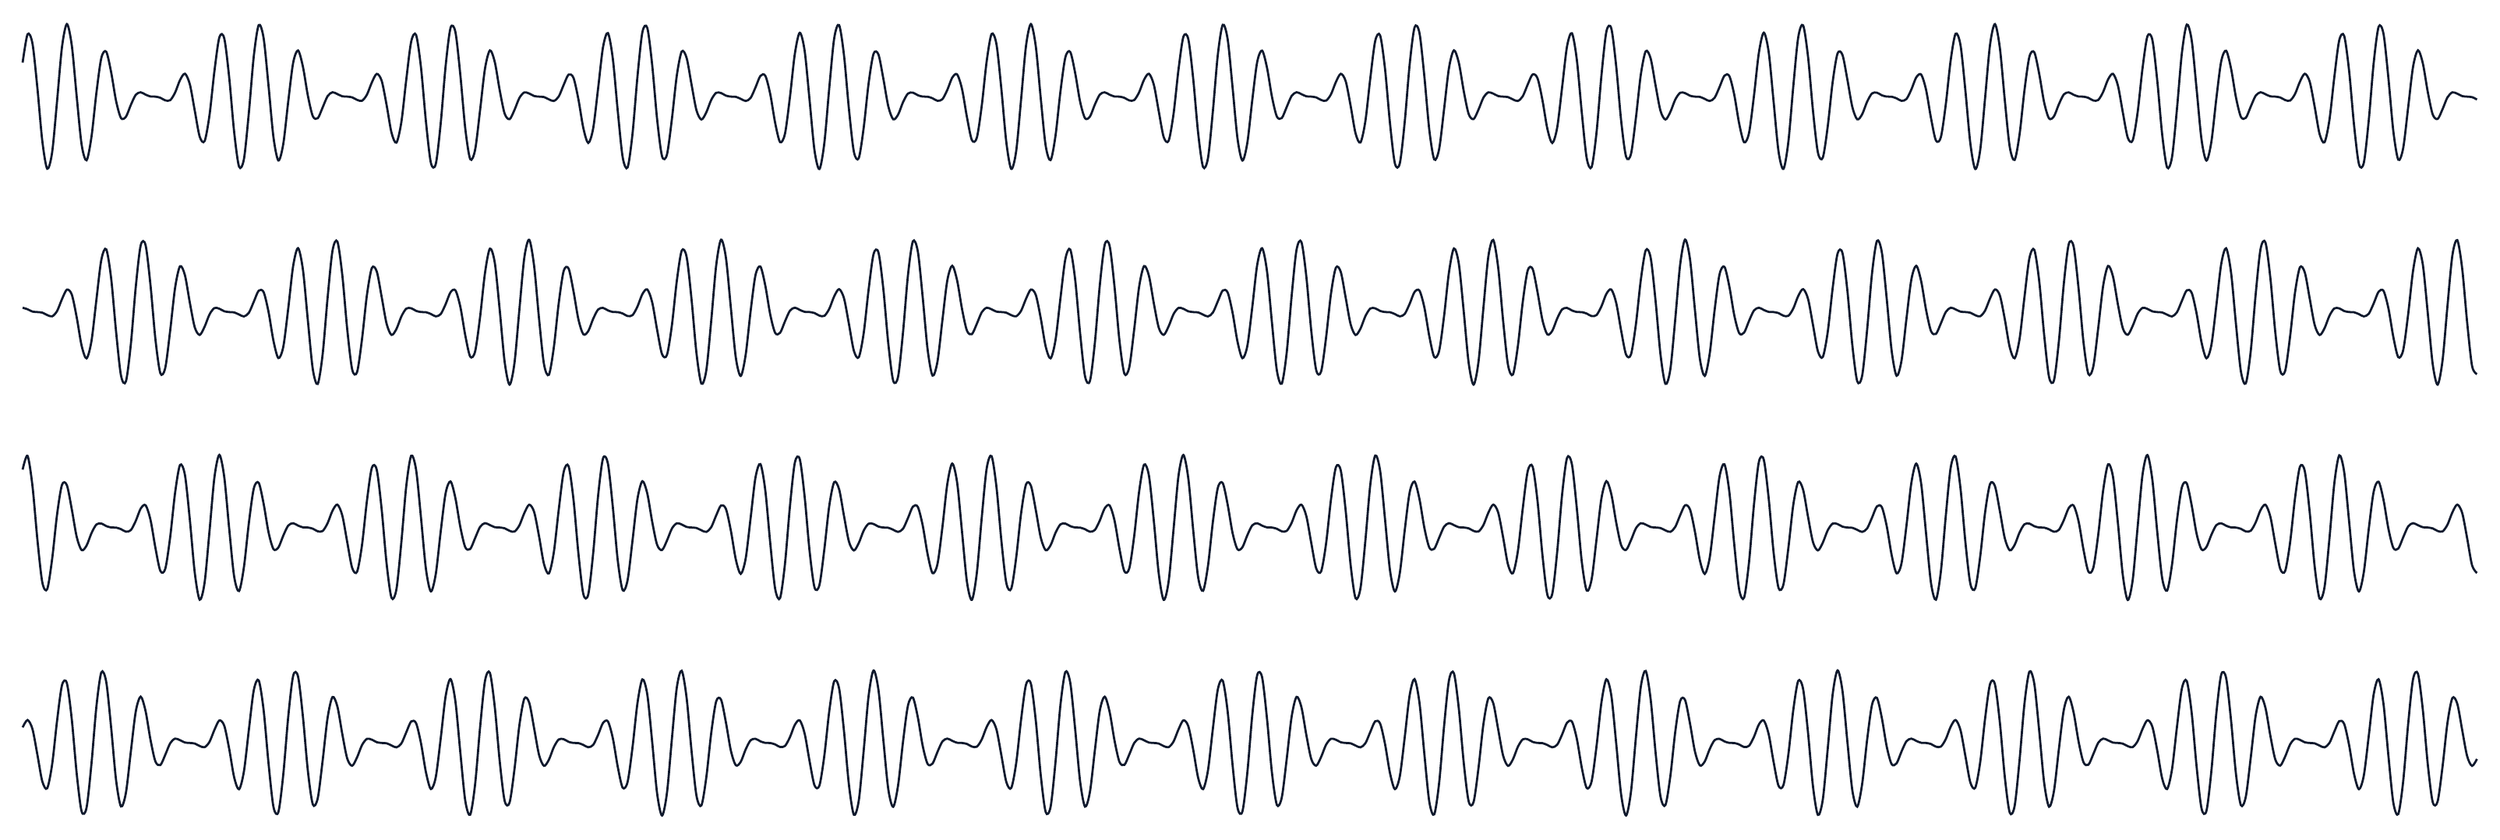
\begin{tikzpicture}{scale=0.9}
  \foreach \shift in {0, 1, ..., 3}
  {
    \draw[
    smooth,
    color=darkBlue,
    line width=1pt,
    smooth,
    yshift=100*\shift,
    domain=-20:20,
    samples=500,
  ] plot (\x, {(exp(-cos(deg(\x-1.9*\shift))*cos(deg(\x-1.9*\shift)))-1) * 1.9 * cos(10 * deg(\x-1.9*\shift) + 90)}); 
  }
    
  % \draw[
  %   color=darkBlue,
  %   line width=1pt,
  %   smooth,
  %   domain=-20:20,
  %   yshift=-100,
  %   xshift=-50,
  %   samples=2000,
  % ] plot (\x, {(exp(-cos(deg(\x))*cos(deg(\x)))-1) * 1.9 * cos(10 * deg(\x) + 90)}); 
  % \draw[
  %   color=lightBlue,
  %   line width=1pt,
  %   smooth,
  %   domain=-20:20,
  %   yshift=-150,
  %   xshift=-50,
  %   samples=2000,
  % ] plot (\x, {(exp(-cos(deg(\x))*cos(deg(\x)))-1) * 1.9 * cos(10 * deg(\x) + 90)}); 
  %\fill[color=lightBlue]
  % \draw[
  %   color=darkBlue,
  %   line width=1pt,
  %   smooth,
  %   yscale=0.9,
  %   xscale=0.57,
  %   xshift=-0.5cm,
  %   yshift=+3cm,
  %   domain=-1.5:9,
  %   samples=200,
  % ] plot (\x, {(exp(-cos(deg(\x))*cos(deg(\x)))-1) * 1.9 * cos(10 * deg(\x) + 90)}); 
\end{tikzpicture}
\end{document}